\documentclass[border=10pt]{standalone}

\usepackage{tikz}
\usepackage{tikzsymbols}
\usetikzlibrary{calc,patterns,shapes.geometric}

\def\centerarc[#1](#2)(#3:#4:#5){\draw[#1] ($(#2)+({#5*cos(#3)},{#5*sin(#3)})$) arc (#3:#4:#5);}

\begin{document}
	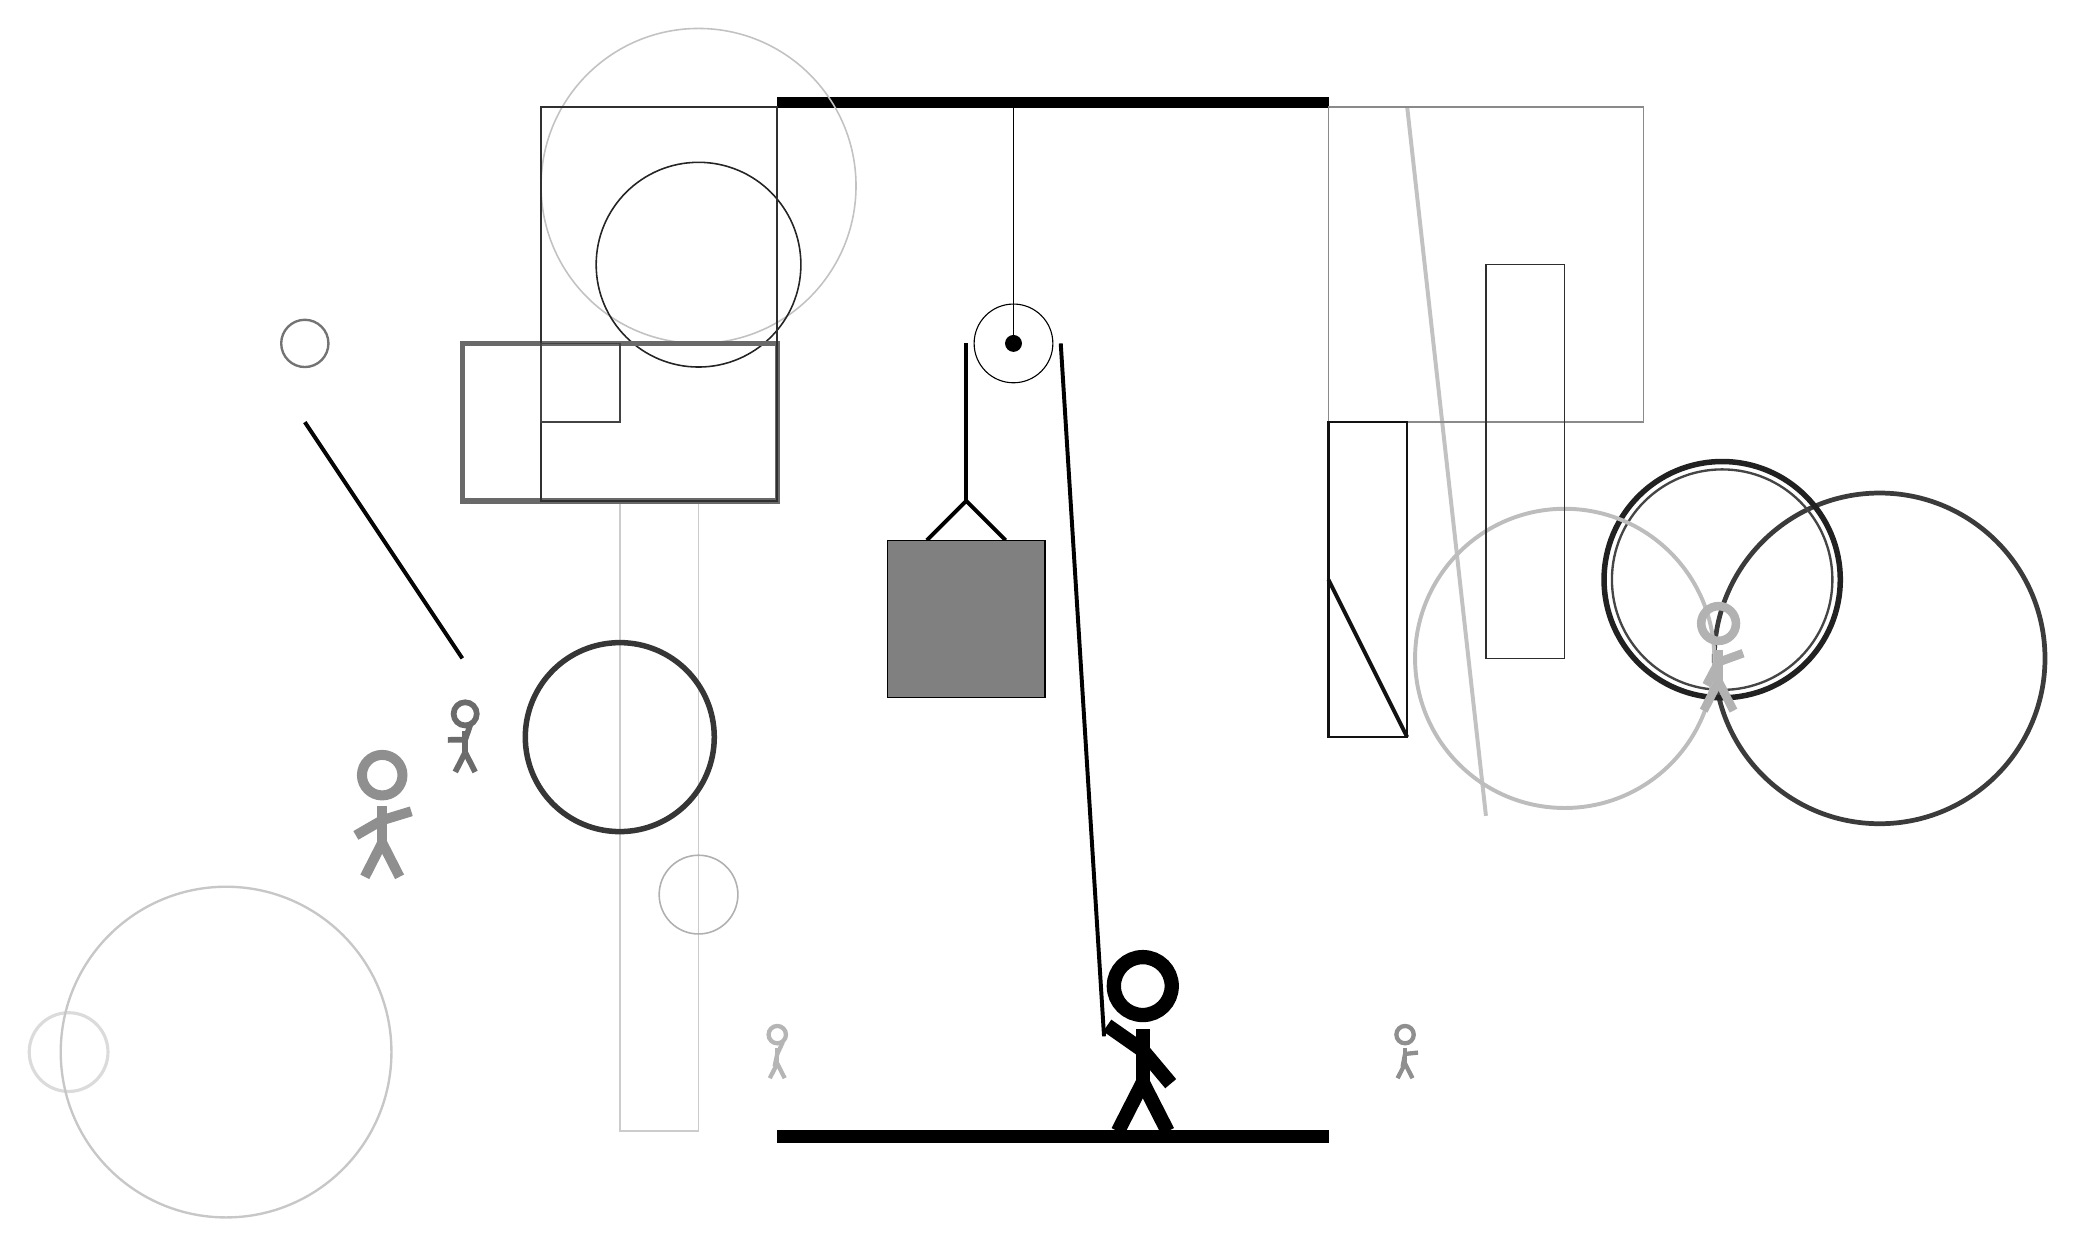
\begin{tikzpicture}
		%%%%% START %%%%%
		
		\draw[fill=black] (-2, 10) rectangle (5, 10.125);
		
		\draw (1, 7) circle (0.5);
		\draw[fill=black] (1, 7) circle (0.1);
		\draw (1, 10) -- (1, 7);
		
		\draw[line width=0.5mm] (-0.1, 4.5) -- (0.4, 5.0) -- (0.9, 4.5);
		\draw[fill=black!50] (-0.6, 4.5) rectangle (1.4, 2.5);
		
		\draw[line width=0.5mm] (0.4, 7) -- (0.4, 5.0);
		\centerarc[line width=0.5mm](1, 7)(0:180:0.6);
		\draw[line width=0.5mm](1.6, 7) -- (2.15, -1.8);
		
		\node at (2.6, -1.9) {\Strichmaxerl[10][-35][-50]};
		
		\node[line width=0.2mm, color=black!29] at (-2, -2) {\Strichmaxerl[3][78][65]};
		
		\draw[line width=0.5mm, color=black!93](6, 2) -- (5, 4);
		\draw[line width=0.2mm, color=black!20] (-3, 5) rectangle (-4, -3);
		\draw[line width=0.5mm, color=black!24](6, 10) -- (7, 1);
		
		\draw[line width=0.2mm, color=black!46] (5, 10) rectangle (9, 6);
		\draw [line width=0.6mm, color=black!77](12, 3) circle (2.1);
		\node[line width=0.6mm, color=black!58] at (-6, 2) {\Strichmaxerl[4][1][71]};
		\draw [line width=0.7mm, color=black!79](-4, 2) circle (1.2);
		\draw [line width=0.7mm, color=black!87](10, 4) circle (1.5);
		
		\draw [line width=0.3mm, color=black!73](10, 4) circle (1.4);
		
		\draw [line width=0.5mm, color=black!26](8, 3) circle (1.9);
		\draw[line width=0.2mm, color=black!82] (7, 8) rectangle (8, 3);
		\draw [line width=0.2mm, color=black!24](-3, 9) circle (2.0);
		
		\draw [line width=0.2mm, color=black!86](-3, 8) circle (1.3);
		\node[line width=0.2mm, color=black!44] at (-7, 1) {\Strichmaxerl[7][30][17]};
		\node[line width=0.7mm, color=black!30] at (10, 3) {\Strichmaxerl[6][62][20]};
		
		\draw[line width=0.7mm, color=black!59] (-2, 5) rectangle (-6, 7);
		
		\draw[line width=0.2mm, color=black!81] (-2, 5) rectangle (-5, 10);
		\draw [line width=0.2mm, color=black!31](-3, 0) circle (0.5);
		
		\draw [line width=0.3mm, color=black!55](-8, 7) circle (0.3);
		\draw[line width=0.5mm, color=black!98](-6, 3) -- (-8, 6);
		
		\node[line width=0.5mm, color=black!44] at (6, -2) {\Strichmaxerl[3][79][6]};
		\draw[line width=0.3mm, color=black!93] (6, 6) rectangle (5, 2);
		\draw [line width=0.4mm, color=black!14](-11, -2) circle (0.5);
		\draw[line width=0.2mm, color=black!74] (-4, 6) rectangle (-5, 7);
		
		\draw [line width=0.3mm, color=black!22](-9, -2) circle (2.1);
		
		\draw[fill=black] (-2, -3) rectangle (5, -3.15);
		
		%%%%% END %%%%%
	\end{tikzpicture}
\end{document}